\documentclass{article}

% if you need to pass options to natbib, use, e.g.:
% \PassOptionsToPackage{numbers, compress}{natbib}
% before loading nips_2016
%
% to avoid loading the natbib package, add option nonatbib:
% \usepackage[nonatbib]{nips_2016}

% \usepackage{nips_2016}

% to compile a camera-ready version, add the [final] option, e.g.:
\usepackage[final]{nips_2016}

\usepackage[utf8]{inputenc} % allow utf-8 input
\usepackage[T1]{fontenc}    % use 8-bit T1 fonts
\usepackage{hyperref}       % hyperlinks
\usepackage{url}            % simple URL typesetting
\usepackage{booktabs}       % professional-quality tables
\usepackage{amsfonts}       % blackboard math symbols
\usepackage{nicefrac}       % compact symbols for 1/2, etc.
\usepackage{microtype}      % microtypography

\usepackage{myTutorialPaper} % imu article
\usepackage{graphicx}
\usepackage{caption}

\title{Nonlinear Data Analytics Final Project}

\author{
  John Kath \\
  \texttt{john.kath@cgu.edu} \\
}

\begin{document}

\maketitle

\tableofcontents

% \begin{abstract}
% \end{abstract}

\section{Project Overview}

\subsection{Description}

\textbf{Project Type (1)}

\begin{enumerate}
  \item Application of existing algorithm to a new problem and
    potentially new data.
\end{enumerate}

\subsection{Requirements}

\begin{itemize}
  \item \textbf{Partner:} Work independently.
  \item \textbf{Dataset:} HMOG cell phone data from 9 
    users / 24 sessions-activities each. Applied data analytics and ML methods using
    accelerometer, gyroscope and magnetometer data (3-axis each).
  \item \textbf{Format:} \LaTeX{} NIPS
  \item \textbf{Code Style:} Used suggested code style guidelines
    (cookiecutter data science) with MIT open-source license.
  \item \textbf{Programming Tools \& Hardware:} Python/Jupyter
    Notebook with Scikit Kinematics library, Matlab with Sensor Fusion and Tracking toolbox.
\end{itemize}

\subsection{Project goals}

This project uses probabilistic models and data analytics methods
introduced in the paper [1] \textit{Using Inertial Sensors for Position
and Orientation Estimation} to estimate the position and orientation
(pose) of a users cell phone during an activity. Kalman filtering fusion algorithms
are used in Matlab and Madgwick's fusion algorithm is used in Scikit Kinematics to predict orientation
of users cell phone during activities.
Cell phone 3D accelerometer, gyroscope and magnetometer data is obtained for
analysis from the HMOG dataset associated with the article [2]
\textit{HMOG: New Behavioral Biometric Features for Continuous
Authentication of Smartphone Users}.

\textbf{The techniques for data analytics used in the project as discussed
in [1] \textit{Using Inertial Sensors for Pose Estimation} are:}

\begin{itemize}
  \item \textbf{(Ch2) Inertial Sensors:} Coordinate frames, angular
    velocity, specific force, sensor error.
  \item \textbf{(Ch3) Probabilistic Models:} Parameterizing/probabilistic
    orientation modeling (Euler angles, Unit quaternions),
    measurement/probabilistic models for pose estimation.
  \item \textbf{(Ch4) Estimating Position and Orientation:} Smoothing
    in optimized frame (Gauss-Newton estimation, uncertainty),
    smoothing estimation of orientation using optimization, filtering
    estimate of orientation using optimization, filtering estimate in
    optimization framework, extended Kalman filtering / complementary
    filtering.
\end{itemize}

\section{Math Models for Pose/Attitude Estimation}

\textbf{NOTE: The following sections restate material from reference [1].}

This section gives the background material and mathematical models used to estimate the orientation of
a device given IMU data. These techniques are applied in both the Matlab Sensor Fusion and Tracking toolbox and
Python Scikit Kinematics library algorithms. These algorithms will be discussed with analysis results in the next
section.

\subsection{HMOG cell phone data}

3D accelerometer, gyroscope and magnetometer data (3 axis each)  [2] HMOG cell phone data for a given user/activity
is used as an input to our pose algorithms. The algorithm output is an estimation of orientation (and possibly position).
Three algorithms for estimating position and orientation will be introduced in the following sections.

\subsubsection{Measurement models}

\textbf{Accelerometer measurement model}

The accelerometer measures the specific force $f^\text{b}_t$ at each time instance~$t$. Our simplified measurement model is
\begin{align}
\label{eq:models-accMeasModel}
y_{\text{a},t} 
= R^{\text{bn}}_t  ( a_{\text{nn}}^\text{n} - g^\text{n} )
+ \delta_{\text{a},t}^\text{b}
+ e_{\text{a},t}^\text{b}.
\end{align} 

\textbf{Gyroscope measurement model}

The gyroscope measures the angular velocity $\omega_{\text{ib}}^\text{b}$ at each time instance $t$. Our simplified
measurement model is
\begin{align}
\label{eq:models-gyrMeasModel}
y_{\omega,t} = \omega_{\text{nb},t}^\text{b} + \delta_{\omega,t}^\text{b} + e_{\omega,t}^\text{b}.
\end{align}

\textbf{Magnetometer measurement model}

Magnetometers measure the local magnetic field, consisting of both the earth magnetic field and the magnetic field due to the presence of magnetic material.
Assuming that the magnetometer only measures the local magnetic field, its measurements $y_{\text{m},t}$ can be modeled as
\begin{align}
\label{eq:models-magMeasModel}
y_{\text{m},t} &= R^\text{bn}_t m^\text{n} + e_{\text{m},t}, 
\end{align}

\subsection{Probabilistic models}

Most complexity in pose estimation lies in the nonlinear nature of the orientation and the fact that orientation can be parametrized in different ways.
When all the measurement data is used in our model this is know as \textit{smoothing}. This is compuation intensive and assumes all measurement data is available
for our estimate. The other class of estimation we will model is know as \textit{filtering}. In filtering we estimate $x_t$ using all measurements up to and including time $t$.

\subsection{Pose estimation}

For pose estimation, we model the accelerometer and gyroscope measurements as inputs to the dynamics. Hence, the state vector consists of the position $p^\text{n}_{t}$, the velocity $v^\text{n}_{t}$ and a parametrization of the orientation. In summary, this leads to the following state space model for pose estimation
\begin{subequations}
\label{eq:models-ssPose}
\begin{align}
\begin{pmatrix} 
p^\text{n}_{t+1} \\
v^\text{n}_{t+1} \\ 
q^\text{nb}_{t+1} 
\end{pmatrix}
&= \begin{pmatrix} 
p_t^\text{n} + T v_t^\text{n} + \tfrac{T^2}{2} \left( R^\text{nb}_t (y_{\text{a},t} - \delta_{\text{a},t}) + g^\text{n} + e_{\text{p,a},t} \right) \\
v_t^\text{n} + T \left( R^\text{nb}_t (y_{\text{a},t}  - \delta_{\text{a},t}) + g^\text{n} + e_{\text{v,a},t} \right) \\
q_t^\text{nb} \odot \expq \left( \tfrac{T}{2} (y_{\omega,t} - \delta_{\omega,t} - e_{\omega,t} ) \right)
\end{pmatrix}, \label{eq:models-ssPose-dyn} \\
y_{\text{p},t} &= p_t^\text{n} + e_{\text{p},t}, \label{eq:models-ssPose-meas}
\intertext{where}
e_{\text{p,a},t} &\sim {\mathrlap{\mathcal{N}(0, \Sigma_\text{a} ),}\phantom{\bar{q}_1^\text{nb} \odot \expq ( \tfrac{e_{\oriError,\text{i}}}{2} )}} \qquad \, e_{\text{v,a},t} \sim \mathcal{N}(0, \Sigma_\text{a} ), \\
e_{\text{p},t} &\sim {\mathrlap{\mathcal{N}(0, \Sigma_\text{p} ),}\phantom{\bar{q}_1^\text{nb} \odot \expq ( \tfrac{e_{\oriError,\text{i}}}{2} ), \, \qquad}} \, e_{\omega,t} \sim \mathcal{N}(0, \Sigma_\omega ), 
\intertext{with $\Sigma_\text{a} = \sigma_\text{a}^2 \, \mathcal{I}_3$ and $\Sigma_\omega = \sigma_\omega^2 \, \mathcal{I}_3$.}
\end{align}
\end{subequations}

\subsection{Orientation estimation}

For orientation estimation, the state vector only consists of a parametrization of the orientation. We use the inertial sensors in combination with the magnetometer measurements to estimate the orientation. This leads to the following state space model for orientation estimation,
\begin{subequations}
\label{eq:models-ssOri}
\begin{align}
q^\text{nb}_{t+1} &= q_t^\text{nb} \odot \expq \left( \tfrac{T}{2} (y_{\omega,t} - \delta_{\omega} - e_{\omega,t} ) \right), \label{eq:models-ssOri-dyn} \\
y_{\text{a},t} &= - R^\text{bn}_t g^\text{n} + e_{\text{a},t} , \label{eq:models-ssOri-measAcc} \\
y_{\text{m},t} &= R^\text{bn}_t m^\text{n} + e_{\text{m},t}, \label{eq:models-ssOri-measMag}
\intertext{where~\eqref{eq:models-ssOri-dyn} describes the dynamics while~\eqref{eq:models-ssOri-measAcc} and~\eqref{eq:models-ssOri-measMag} describe the measurement models and} 
e_{\omega,t} &\sim \mathcal{N}(0,\Sigma_\omega), \qquad e_{\text{a},t} \sim \mathcal{N}(0, \Sigma_\text{a}), \qquad e_{\text{m},t} \sim \mathcal{N}(0,\Sigma_\text{m}),
\end{align}
\end{subequations}
with $\Sigma_\omega = \sigma_\omega^2 \, \mathcal{I}_3$ and $\Sigma_\text{a} = \sigma_\text{a}^2 \, \mathcal{I}_3$. The initial orientation is given by the QUEST algorithm.

\subsection{Estimating position and orientation}

We will focus on position and orientation estimation using the probabilistic models developed. Algorithm 1 is a orientation estimate based on a smoothing. Algorithms 2 and 3 use filtering to estimate orientation. Our focus will be orientation estimation problems since they illustrate the most important parts of the pose estimation. Most complexities lie in the parametrization of the orientation and in the nonlinear nature of the orientation.

\subsection{Gauss-Newton optimization}

\label{sec:oriEst-GNopt}
To obtain a smoothing estimate of the position and orientation using optimization, we first recognize that for our models~\eqref{eq:models-ssPose} and~\eqref{eq:models-ssOri}, all probability distributions are Gaussian. Let us therefore consider a slightly more general problem where the objective function consists of the product of Gaussian probability functions $p(e_i(x_{1:N}))$, $i = 1, \hdots, M$. Hence, the optimization problem can be written as
\begin{align}
\hat{x}_{1:N} = \argmin_{x_{1:N}} - \sum_{i = 1}^M \log p \left(e_i (x_{1:N}) \right). \label{eq:oriEst-optNegLogLikGaussian}
\end{align}
The probability distribution of $e_i(x)$ is given by
\begin{align}
p \left(e_i(x_{1:N}) \right) = \tfrac{1}{\sqrt{ (2 \pi)^{n_e} \det \Sigma_i}} \exp \left( - \tfrac{1}{2} e_i^\Transp(x_{1:N}) \Sigma_i^{-1} e_i(x_{1:N}) \right).
\end{align}
Omitting the terms independent of $x_{1:N}$, the optimization problem~\eqref{eq:oriEst-optNegLogLikGaussian} reduces to
\begin{align}
\label{eq:oriEst-generalNLS}
\hat x_{1:N} = \argmin_{x_{1:N}} \tfrac{1}{2} \sum_{i = 1}^M \| e_i(x_{1:N}) \|_{\Sigma_i^{-1}}^2, 
\end{align}
with $\| e_i(x_{1:N}) \|_{\Sigma_i^{-1}}^2 = e^\Transp_i(x_{1:N}) \Sigma_i^{-1} e_i(x_{1:N})$. The function that is being minimized in optimization problems, is often referred to as the \emph{objective function}.

The solution to~\eqref{eq:oriEst-generalNLS} can be found by studying the shape of the objective function as a function of $x_{1:N}$. This can be characterized in terms of the \textit{gradient} $\mathcal{G}(x_{1:N})$ and \textit{Hessian} $\mathcal{H}(x_{1:N})$, which provide information about the slope and curvature of the function, respectively. Defining 
\begin{align*}
e^\Transp_i(x_{1:N}) \Sigma_i^{-1} e_i(x_{1:N}) = \varepsilon_i^\Transp \varepsilon_i, \qquad \varepsilon_i = \Sigma_i^{-1/2} e_i(x_{1:N}),
\end{align*}
and the stacked variables 
\begin{align*}
\varepsilon = \begin{pmatrix} \varepsilon_1^\Transp & \cdots & \varepsilon^\Transp_M \end{pmatrix}^\Transp,
\end{align*}
the gradient and the Hessian are given by
\begin{subequations}
\label{eq:oriEst-gradHess}
\begin{align}
\mathcal{G}(x_{1:N}) &= \sum_{i = 1}^{M} \left( \tfrac{\diff \varepsilon_i}{\diff x_{1:N}} \right)^\Transp \varepsilon_i= \mathcal{J}^\Transp(x_{1:N}) \varepsilon, \label{eq:oriEst-gradient} \\
\mathcal{H}(x_{1:N}) &= \sum_{i = 1}^{M} \left( \left( \tfrac{\diff \varepsilon_i}{\diff x_{1:N}} \right)^\Transp \tfrac{\diff \varepsilon_i}{\diff x_{1:N}} + \varepsilon_i^\Transp \tfrac{\diff^2 \varepsilon_i}{\diff x_{1:N}^2} \right) \nonumber \\
&= \mathcal{J}^\Transp(x_{1:N}) \mathcal{J}(x_{1:N}) + \sum_{i = 1}^{M} \varepsilon_i^\Transp \tfrac{\diff^2 \varepsilon_i}{\diff x_{1:N}^2}. \label{eq:oriEst-hessian}
\end{align}
\end{subequations}
Note that for notational convenience, we have omitted the explicit dependence of~$\varepsilon$ on $x_{1:N}$. In~\eqref{eq:oriEst-gradHess}, we introduced the notation $\mathcal{J}(x_{1:N})$, which is the \emph{Jacobian} of the vector $\varepsilon$ with respect to $x_{1:N}$ as
\begin{align}
\mathcal{J}(x_{1:N}) = \begin{pmatrix} \tfrac{\diff \varepsilon_1}{\diff x_1} & \hdots & \tfrac{\diff \varepsilon_1}{\diff x_N} \\
\vdots & & \vdots \\
\tfrac{\diff \varepsilon_{M n_\varepsilon}}{\diff x_1} & \hdots & \tfrac{\diff \varepsilon_{ M n_\varepsilon}}{\diff x_N}
\end{pmatrix},
\end{align}
where $n_\varepsilon$ is the length of the vector $\varepsilon_i$. Instead of computing the true Hessian~\eqref{eq:oriEst-hessian}, we compute an approximation of it given by
\begin{align}
\label{eq:oriEst-approxHessian}
\mathcal{\hat{H}}(x_{1:N}) = \mathcal{J}^\Transp(x_{1:N}) \mathcal{J}(x_{1:N}).
\end{align}
This has the benefit of not having to compute second derivatives, at the same time as it guarantees that the Hessian is positive semidefinite. The downside of using~\eqref{eq:oriEst-approxHessian} is that it introduces an approximation.

The gradient and the (approximate) Hessian can be used to find the minimum of the objective function. For our models~\eqref{eq:models-ssPose} and~\eqref{eq:models-ssOri}, in which the functions $e_i(x_{1:N})$ are nonlinear, an estimate $\hat{x}_{1:N}$ can iteratively be computed as
\begin{align}
\label{eq:oriEst-GNiteration}
\hat x_{1:N}^{(k+1)} = \hat x_{1:N}^{(k)} - \beta^{(k)} \left( \mathcal{\hat{H}}(\hat x_{1:N}^{(k)}) \right)^{-1} \mathcal{G}(\hat x_{1:N}^{(k)}),
\end{align}
where $k$ denotes the iteration number. The \emph{step length} $\beta^{(k)}$ is computed for instance using a backtracking line search. The \emph{search direction} is computed as $\left( \mathcal{\hat{H}}(\hat x_{1:N}^{(k)}) \right)^{-1} \mathcal{G}(\hat x_{1:N}^{(k)})$. Note that an initial point $\hat{x}_{1:N}^{(0)}$ needs to be chosen close enough to the desired minimum to ensure convergence to this minimum. 

At each Gauss-Newton iteration~\eqref{eq:oriEst-GNiteration}, we estimate the state vector $\oriError_{1:N}^\text{n}$. Before starting the next iteration, the linearization points $\tilde{q}^\text{nb}_{1:N}$ are updated and the state vector $\oriError_{1:N}^\text{n}$ is reset to zero.

\subsection{Computing the uncertainty}

We are not only interested in obtaining point estimates of the position and orientation, but also in estimating their uncertainty.
We can therefore approximate the covariance of our estimates as
\begin{align}
\cov{ (\hat{x}_{1:N}) } = \left( \mathcal{J}^\Transp(\hat{x}_{1:N}) \mathcal{J}(\hat{x}_{1:N}) \right)^{-1}.
\end{align}

\subsection{Smoothing estimation algorithms}

\textit{Algorithm 1} details the steps necessary to apply the Gauss-Newton optimization method to obtain
a smoothing estimate of orientation with associated error covariance.

\begin{algorithm}[ht]
  \caption{\textsf{Smoothing estimates of the orientation using optimization}}
  \label{alg:oriEst-smoothingOpt}
  \small
  \textsc{Inputs:} An initial estimate of the orientation $\tilde{q}^{\text{nb},(0)}_{1:N}$, inertial data $\left\{ y_{\text{a},t}, y_{\omega,t} \right\}_{t=1}^N$, magnetometer data $\left\{ y_{\text{m},t}\right\}_{t=1}^N$ and covariance matrices $\Sigma_\omega$, $\Sigma_\text{a}$ and $\Sigma_\text{m}$. \\
  \textsc{Outputs:} An estimate of the orientation $\hat{q}^\text{nb}_{1:N}$ and optionally its covariance $\cov (\hat{\oriError}^\text{n}_{1:N})$.
  \algrule[.4pt]
  \begin{enumerate}
  \item Set $\hat \oriError_t^{\text{n},(0)} = 0_{3 \times 1}$ for $t = 1, \hdots, N$, set $k = 0$ and compute $\initEst{q}_1^\text{nb}$ and $\Sigma_{\oriError,\text{i}}$.
  \item \textbf{while} \textit{termination condition is not satisfied} \textbf{do}
  \begin{enumerate}
  \item Compute the gradient~\eqref{eq:oriEst-gradient} and the approximate Hessian~\eqref{eq:oriEst-approxHessian} of the orientation smoothing problem using the expressions for the different parts of the cost function and their Jacobians.
  \item Apply the update~\eqref{eq:oriEst-GNiteration} to obtain $\hat \oriError_{1:N}^{\text{n},(k+1)}$.
  \item Update the linearization point as
  \begin{align}
  \tilde q^{\text{nb},(k+1)}_t = \expq \left( \tfrac{\hat{\oriError}_t^{\text{n},(k+1)}}{2} \right) \odot \tilde{q}^{\text{nb},(k)}_t,
  \label{eq:oriEst-relinSmoothing}
  \end{align}
  and set $\hat \oriError_t^{\text{n},(k+1)} = 0_{3 \times 1}$ for $t = 1, \hdots, N$.
  \item Set $k = k+1$.
  \end{enumerate}
  \item[] \textbf{end while}
  \item Set $\hat{q}^\text{nb}_{1:N} = \tilde{q}^{\text{nb},(k)}_{1:N}$.
  \item Optionally compute
  \begin{align}
  \cov (\hat{\oriError}^\text{n}_{1:N}) = \left( \mathcal{J}^\Transp(\hat{\oriError}^\text{n}_{1:N}) \mathcal{J} (\hat{\oriError}^\text{n}_{1:N}) \right)^{-1}.
  \end{align}
  \end{enumerate}
  \normalsize
\end{algorithm}

\subsection{Filtering estimation algorithms}

\textit{Algorithm 2 (this is Algorithm 3 in referenced article [1])} details the steps necessary to
obtain the Kalman filtering estimate of orientation with associated error covariance.

\begin{algorithm}[ht]
  \caption{\textsf{Orientation estimation using an EKF with quaternion states}}
  \label{alg:oriEst-ekfQuat}
  \small
  \textsc{Inputs:} Inertial data $\left\{ y_{\text{a},t}, y_{\omega,t} \right\}_{t=1}^N$, magnetometer data $\left\{ y_{\text{m},t}\right\}_{t=1}^N$ and covariance matrices $\Sigma_\omega$, $\Sigma_\text{a}$ and $\Sigma_\text{m}$. \\
  \textsc{Outputs:} An estimate of the orientation $\hat{q}^\text{nb}_{t \mid t}$ and its covariance $P_{t \mid t}$ for $t = 1, \hdots N$.
  \algrule[.4pt]
  \begin{enumerate}
  \item Compute $\initEst{q}^\text{nb}_{1}$ and $\Sigma_\text{i}$ as described in \Sectionref{sec:models-prior} and set $\hat{q}_{1 \mid 1}^\text{nb} = \initEst{q}_{1}^\text{nb}$ and $P_{1 \mid 1} = \Sigma_\text{q,i}$.
  \item \textbf{For} $t = 2, \hdots, N$ \textbf{do}
  \begin{enumerate}
  \item Time update
  \begin{subequations}
  \begin{align}
  \hat{q}^\text{nb}_{t \mid t-1} &= \hat{q}^\text{nb}_{t-1 \mid t-1} \odot \expq \left( \tfrac{T}{2} y_{\omega,t-1} \right), \\
  P_{t \mid t-1} &= F_{t-1} P_{t-1 \mid t-1} F_{t-1}^\Transp + G_{t-1} Q G_{t-1}^\Transp, \label{eq:quatEKF_TPupdate} %
  \end{align}%
  \label{eq:ori_qEkf_timeUpdate}%
  \end{subequations}%
  with $Q = \Sigma_\omega$ and 
  \begin{align*}
  F_{t-1} = \left( \expq (\tfrac{T}{2} y_{\omega,t-1}) \right)^\rightMult, \, G_{t-1} = -\tfrac{T}{2} \left( \hat{q}^{\text{nb}}_{t-1 \mid t-1} \right)^\leftMult \tfrac{\diff \expq (e_{\omega,t-1})}{\diff e_{\omega,t-1}}.
  \end{align*}
  \item Measurement update
  \begin{subequations}
  \begin{align}
  \tilde{q}^\text{nb}_{t \mid t} &= \hat{q}^\text{nb}_{t \mid t-1} + K_t \varepsilon_t,  \\
  \tilde{P}_{t \mid t} &= P_{t \mid t-1} - K_t S_t K_t^\Transp, 
  \end{align}
  \label{eq:ori_qEkf_measUpdate}
  \end{subequations}%
  with $\varepsilon_t$, $K_t$ and $S_t$ defined in~\eqref{eq:oriEst-defEpsKS} and
  \begin{align*}
  y_t &= \begin{pmatrix} y_{\text{a},t} \\ y_{\text{m},t} \end{pmatrix}, & 
  \hat{y}_{t \mid t-1} &= \begin{pmatrix} -\hat{R}^\text{bn}_{t \mid t-1} g^\text{n} \\ \hat{R}^\text{bn}_{t \mid t-1} m^\text{n} \end{pmatrix}, \\
  H_t &= \begin{pmatrix} - \left. \tfrac{\partial R^\text{bn}_{t \mid t-1}}{\partial q^\text{nb}_{t \mid t-1}} \right|_{q^\text{nb}_{t \mid t-1}=\hat{q}^\text{nb}_{t \mid t-1}} g^\text{n} \\ \left. \tfrac{\partial R^\text{bn}_{t \mid t-1}}{\partial q^\text{nb}_{t \mid t-1}} \right|_{q^\text{nb}_{t \mid t-1}=\hat{q}^\text{nb}_{t \mid t-1}} m^\text{n} \end{pmatrix}, & 
  R &= \begin{pmatrix} \Sigma_\text{a} & 0 \\ 0 & \Sigma_\text{m} \end{pmatrix}.
  \end{align*}
  \item Renormalize the quaternion and its covariance as
  \begin{align}
  \hat{q}_{t \mid t}^\text{nb} = \tfrac{\tilde{q}^\text{nb}_{t \mid t}}{\| \tilde{q}^\text{nb}_{t \mid t}\|_2} , \qquad
  P_{t \mid t} = J_t \tilde{P}_{t \mid t} J_t^\Transp,
  \end{align}
  with $J_t = \tfrac{1}{\| \tilde{q}^\text{nb}_{t \mid t} \|_2^3} \tilde{q}^\text{nb}_{t \mid t} \left( \tilde{q}^\text{nb}_{t \mid t} \right)^\Transp$.
  \end{enumerate}
  \item[] \textbf{end for}
  \end{enumerate}
  \normalsize
\end{algorithm}

\pagebreak

\section{Analysis Results}

We will be comparing HMOG user cell phone orientation estimates for two kinds of attitude and heading reference system (AHRS) algorithms: Kalman filters and Madgwick \& Mahony filtering. These algorithms are know as \textit{fusion algorithms} because they fuse accelerometer, gyroscope and magnetometer measurements to produce the optimal estimate of a devices orientation. The goal of these filters is to remove error introduced by IMU sensor measurements in the form of bias, drift and noise.

The gyroscope measures the angular rate of a moving object, the accelerometer measures the acceleration of a certain object, and the magnetometer measures the magnetic field. However, low-cost sensors have inherent drawbacks such as nonlinearity, random walk, temperature drift, etc. In order to obtain a reliable attitude solution, magnetic and inertial measurement unit (MIMU) sensor measurements have to be fused together using optimal sensor fusion algorithms. There are mainly two different fusion approaches. One category includes the \textit{complementary filters} and the other relates to \textit{Kalman filtering}.

\subsection{IMU sensor measurements}

\textbf{Axes definitions} Device is equipped with three-axis accelerometer, gyroscope and vector magnetometer with mutually orthogonal axes: x axis is looking “forward”, z axis is looking “downwards”, y axis completes the right orthogonal system of axes.

\textbf{Gyroscope} measures positive angular rates being rotated counter-clockwise (if one watches from the end of the corresponding axis) in $rad/sec$.

\textbf{Accelerometer} measures the gravity force (it actually doesn’t - it can only measure active forces, and when it sits on the table it measures the force with which the table acts on the accelerometer body preventing it from falling right through the lid of the table) in $m/sec^{2}$.

\textbf{Magnetometer} measures the Earth’s magnetic field vector in $micro-tesla$.

\begin{figure}[t]
  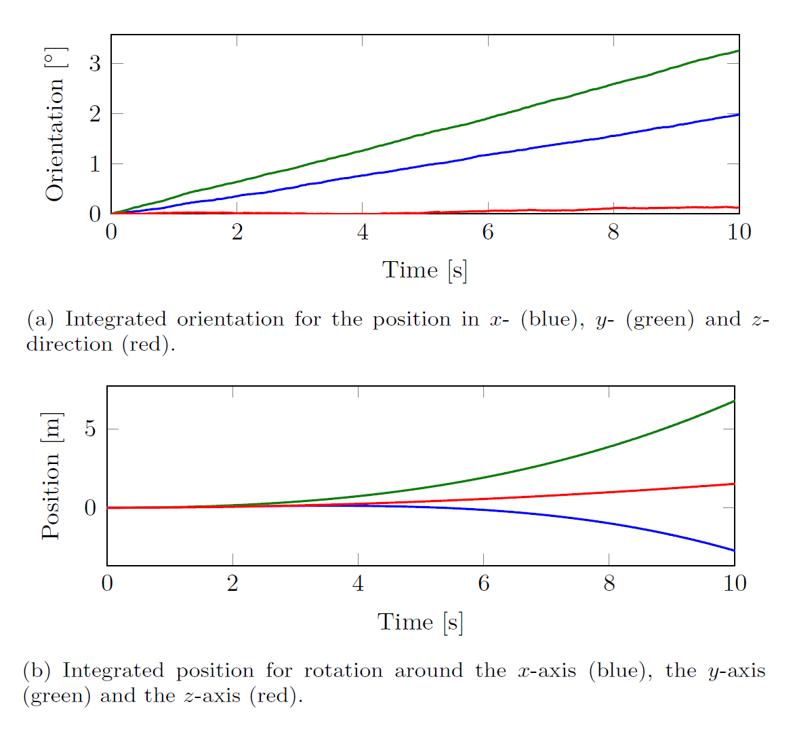
\includegraphics[width=1\linewidth]{images/integration_drift.png}
  \caption[]{Integration drift.}
  %
  \label{fig:IntegrationDrift}
\end{figure}

\subsection{IMU sensor errors}

Integration of the gyroscope measurements provides information about the orientation of the sensor. After subtraction of the earth's gravity, double integration of the accelerometer measurements provides information about the sensor's position. To be able to subtract the earth's gravity, the orientation of the sensor needs to be known. Hence, estimation of the sensor's position and orientation are inherently linked when it comes to inertial sensors.

The process of integrating the measurements from inertial sensors to obtain position and orientation information, is called \textit{deadreckoning}.

Inertial measurements are noisy and biased. Because of this, the integration steps from angular velocity to rotation and from acceleration to position introduce \textit{integration drift}.

Accelerometers can itself measure the inclination, they have a slow response. Gyros measure angle rate change, fast response but the problems for gyros is the zero drift and it has to be compensated for any usable application.

While at steady state, a filter is used such that accelerometers track and eliminate the gyro drift in the vertical plane, where the gravity vector is used for inclination (roll, pitch), but in horizontal plane heading/yaw there is not such possibility, therefore magnetometer can be used. A magnetometer is mainly used for speed detection and with fusion algorithm it can eliminate the gyro offset.

\subsection{Matlab Sensor Fusion and Tracking Toolbox}

The Matlab Ahrsfilter and Imufilter algorithms were used to estimate orientation for 9 HMOG cell phone users 24 sessions each. Results for 3 users (single session each) are shown below.

\begin{figure}[ht] %t
  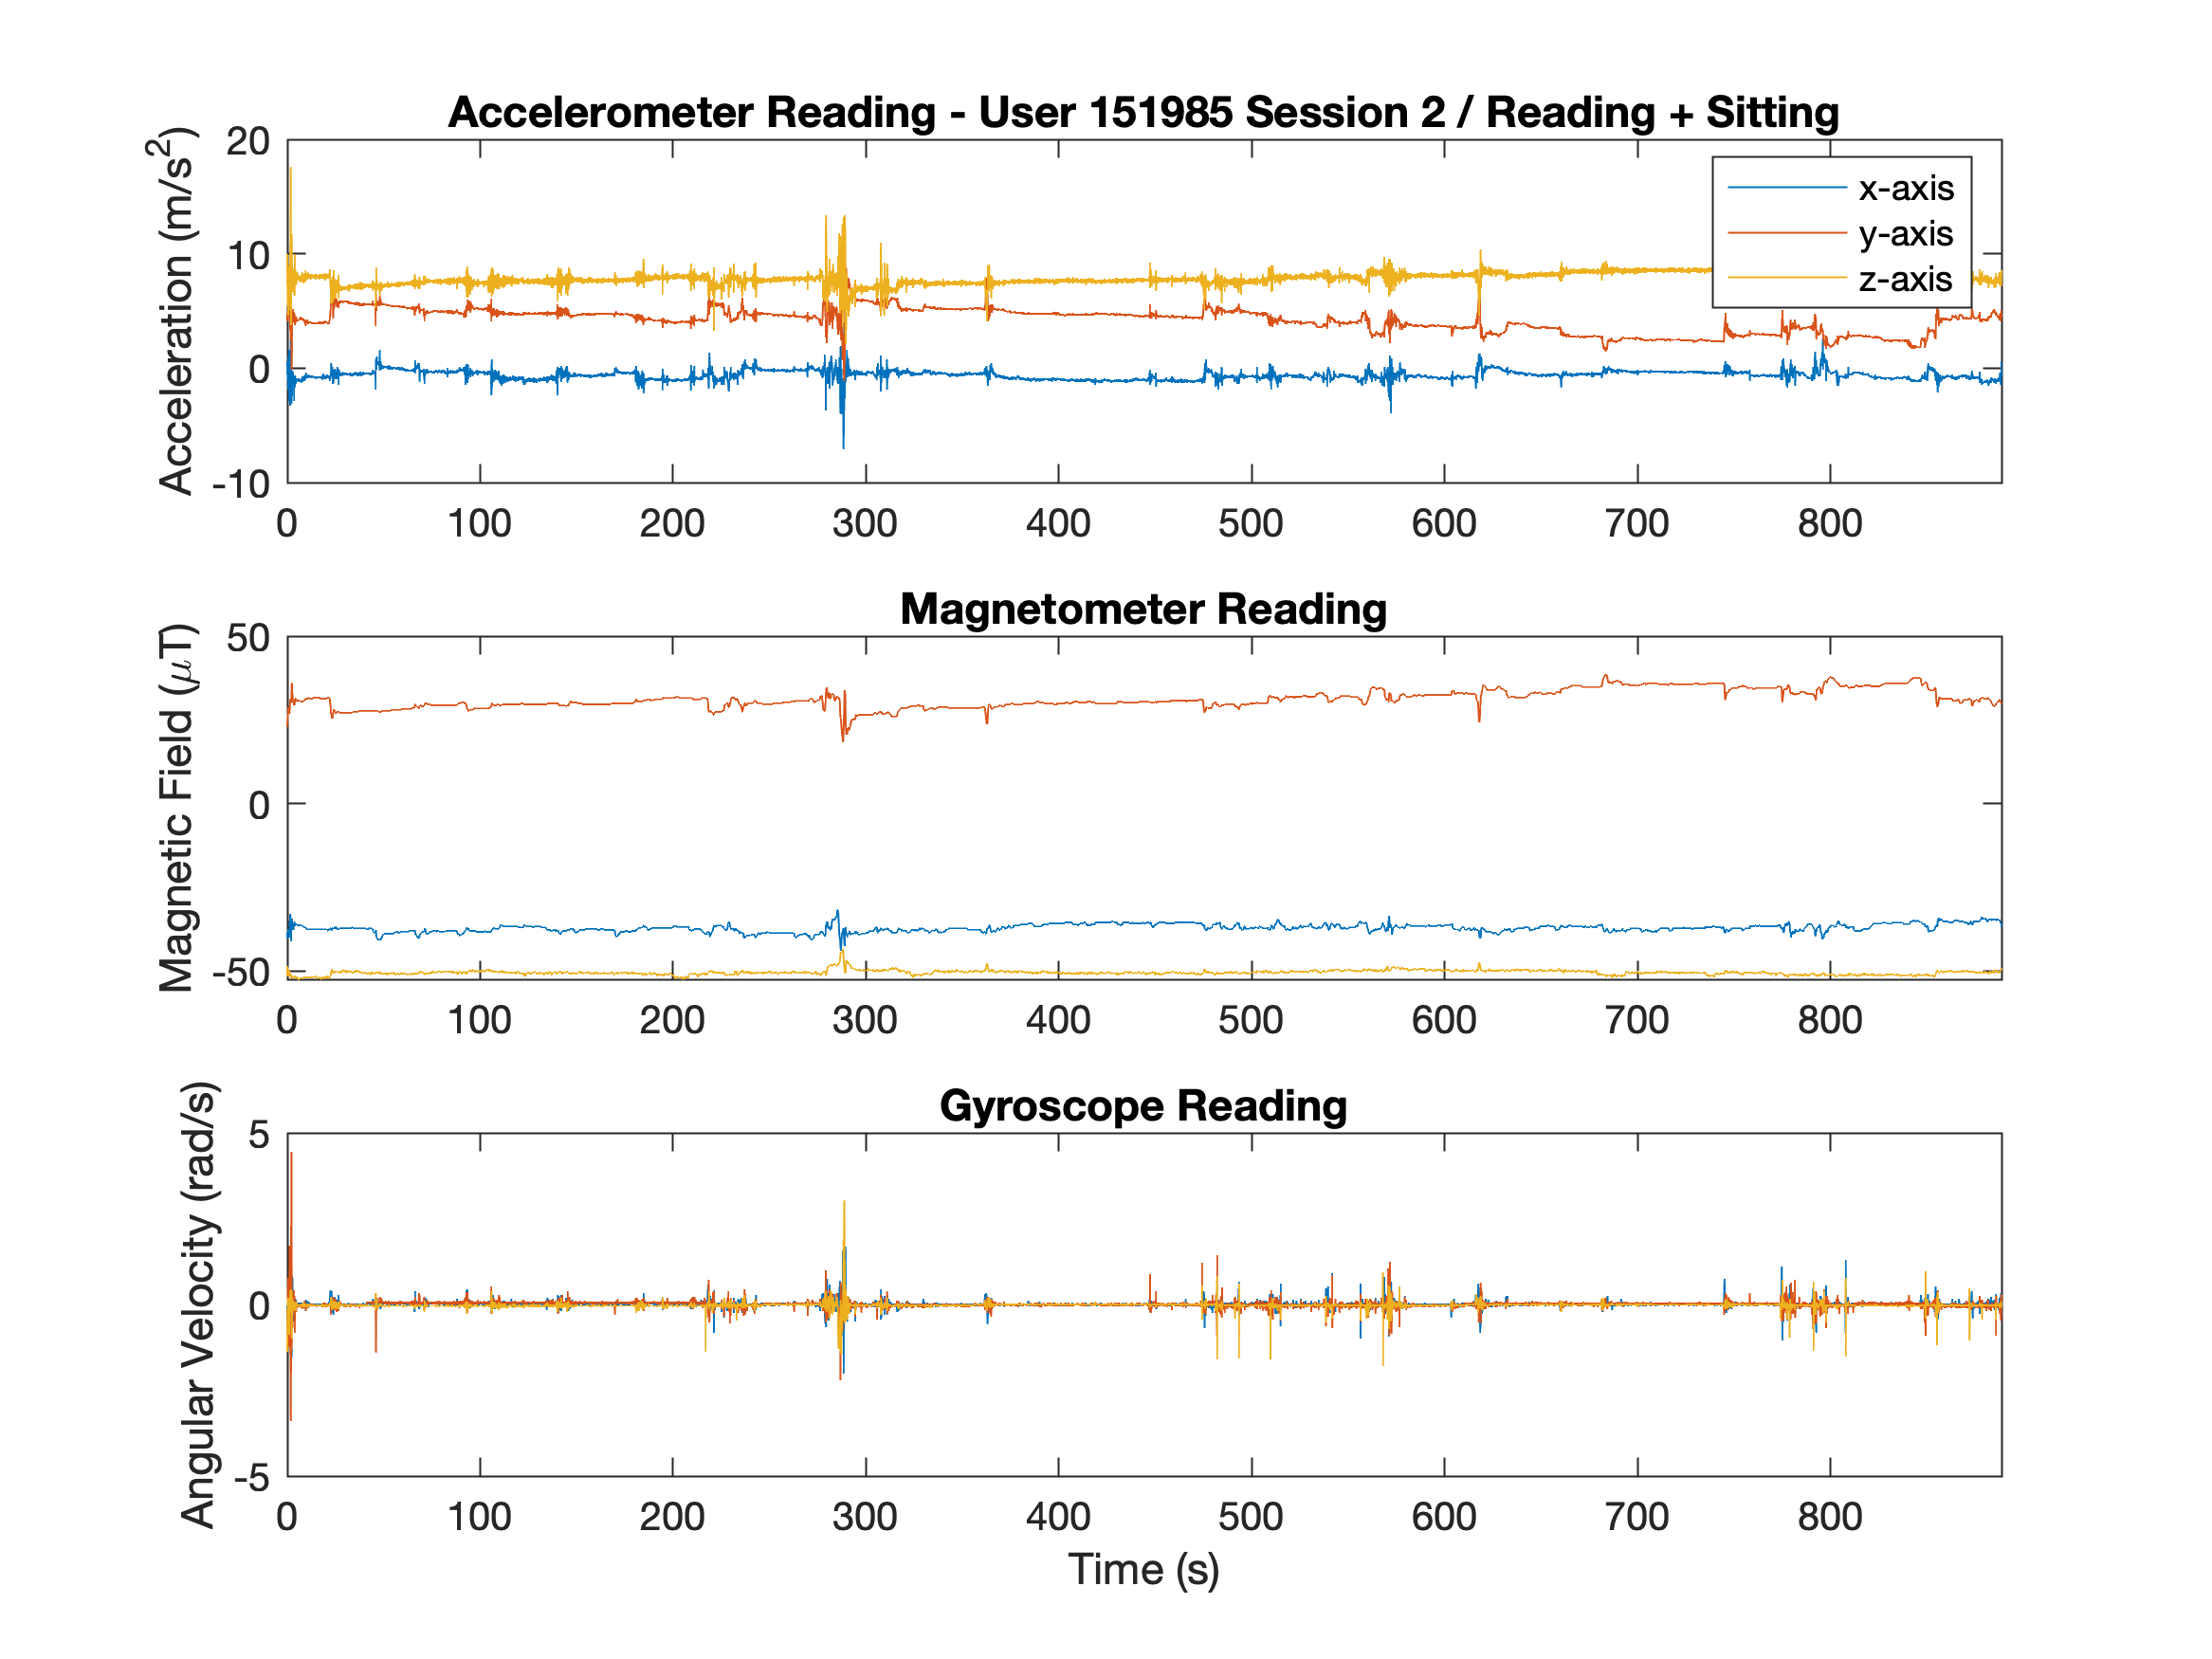
\includegraphics[width=1\linewidth]{images/151985_2_acc_mag_gyr_data.png}
  \caption[]{HMOG cell phone IMU data.}
  %
  \label{fig:151985_2_imu}
\end{figure}

\begin{figure}[ht]
  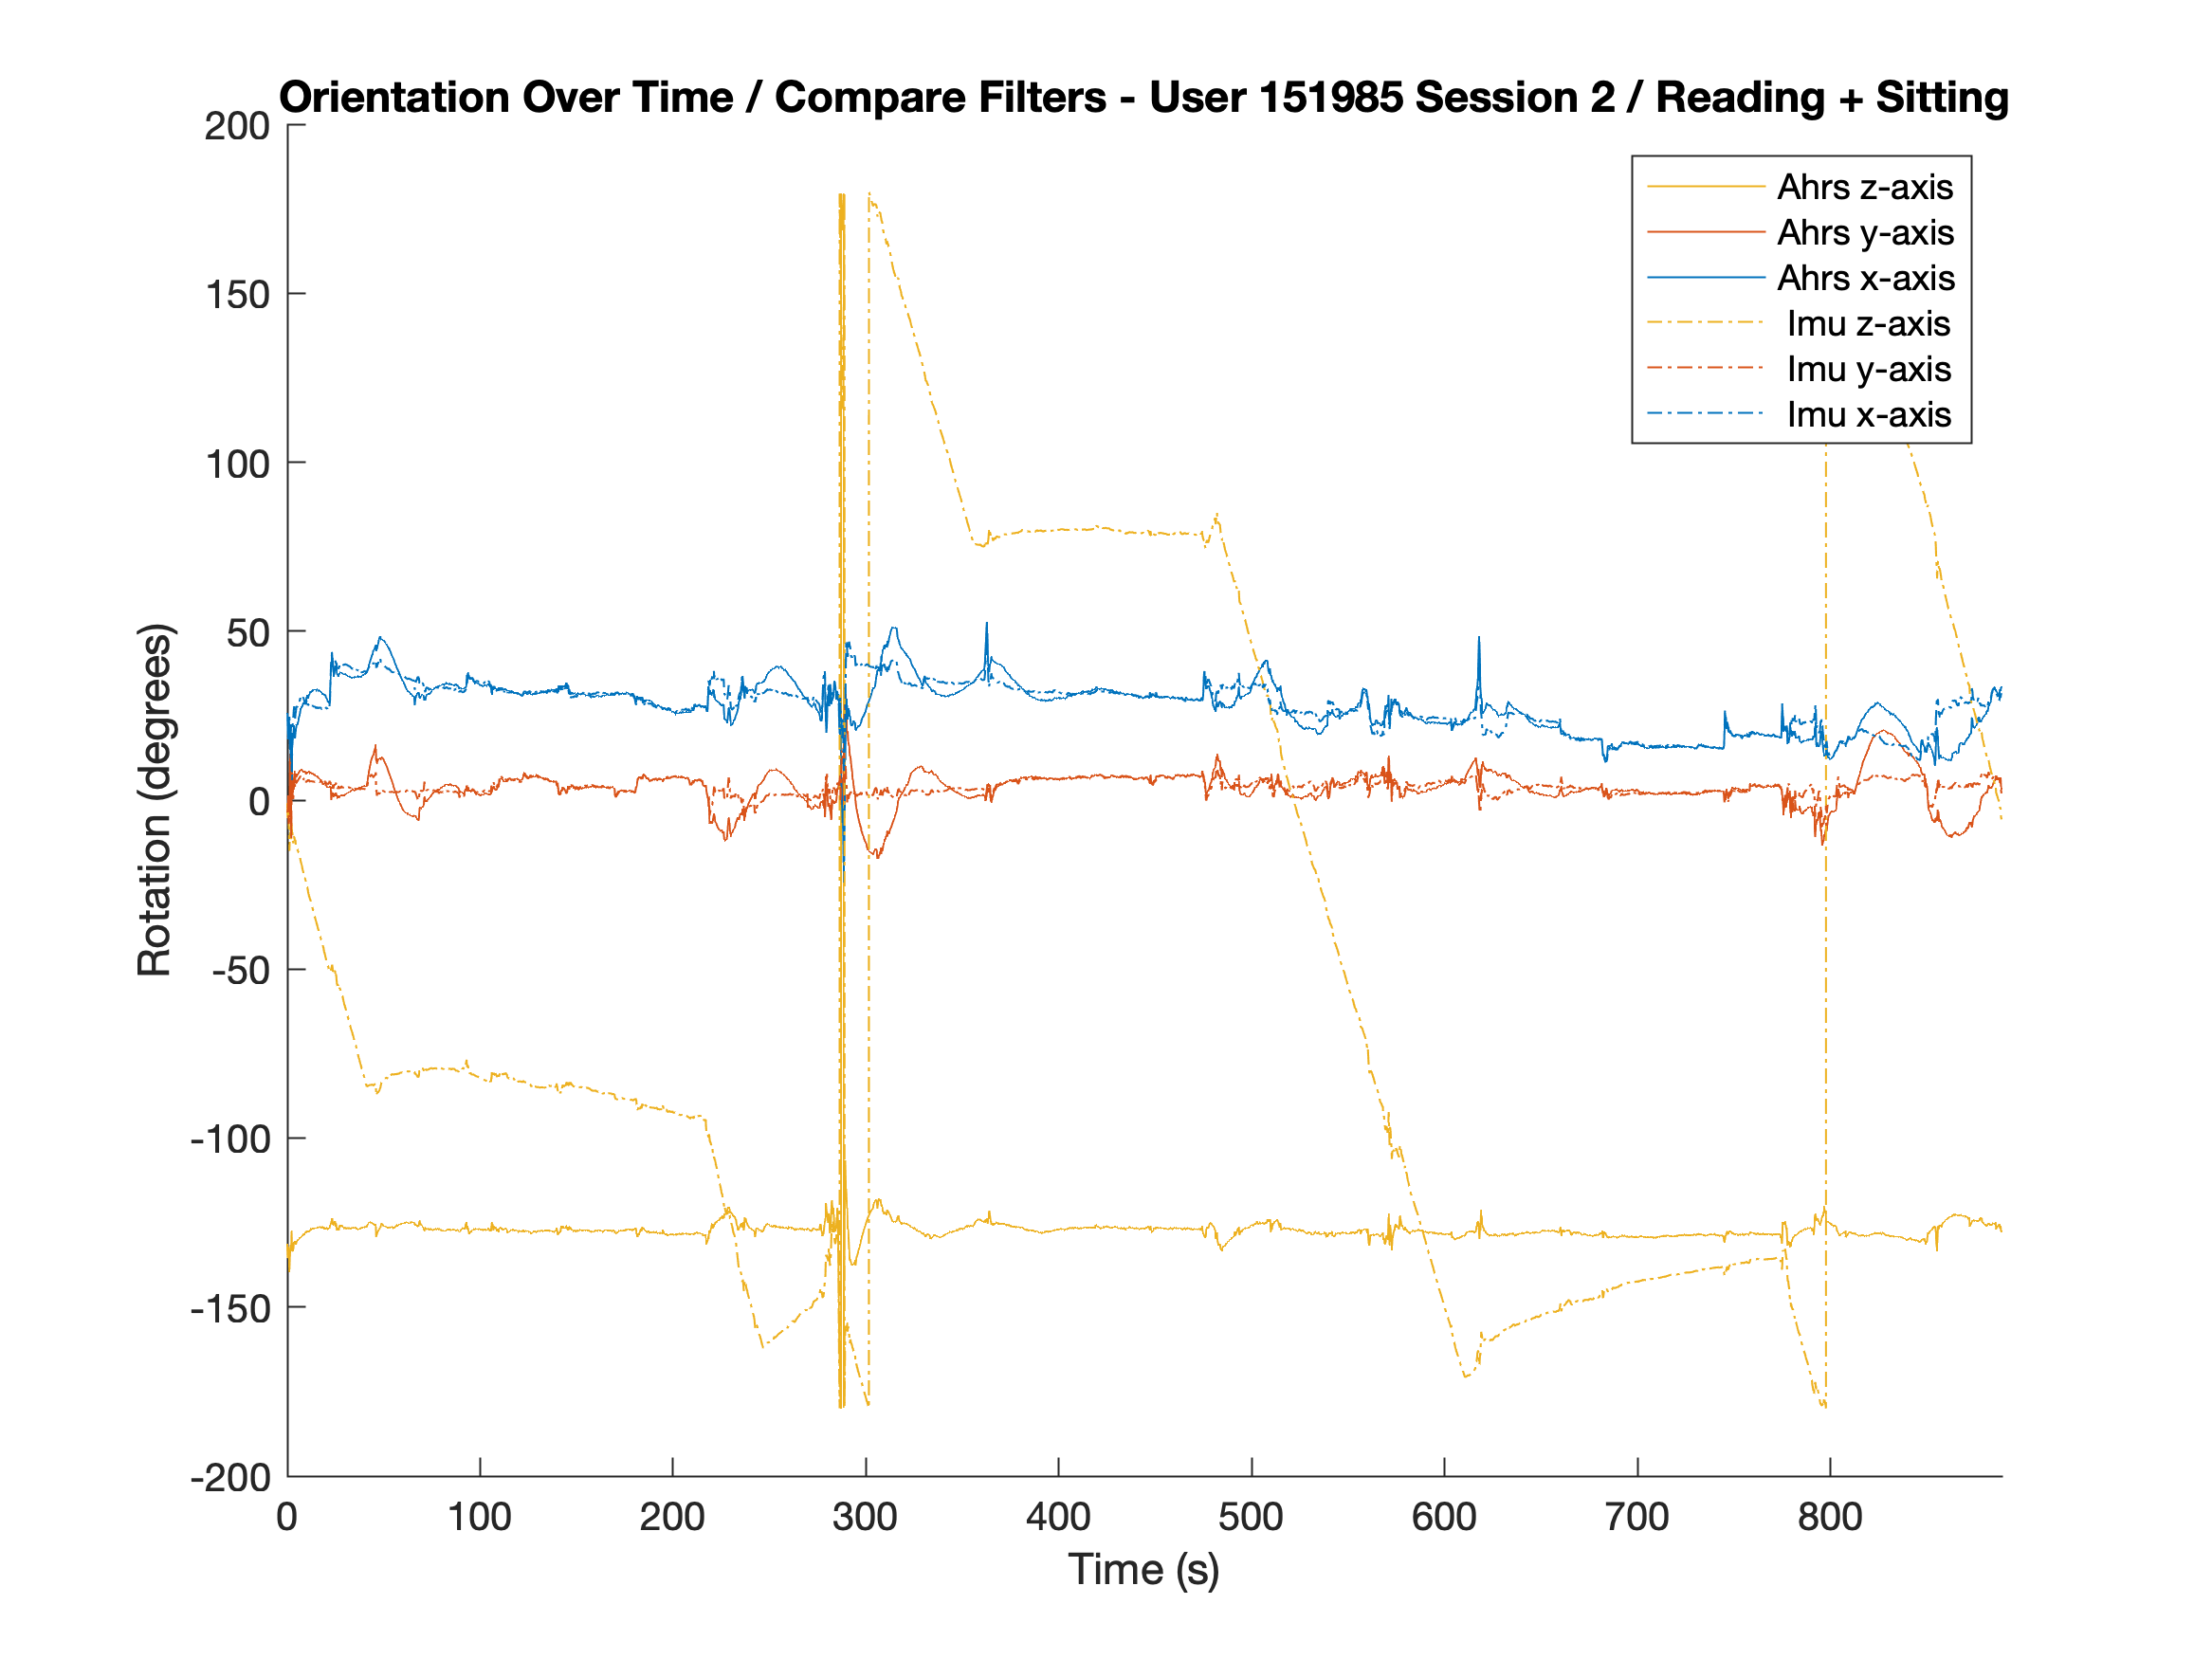
\includegraphics[width=1\linewidth]{images/151985_2_orientation_compare_filters.png}
  \caption[]{Comparison Matlab AHRS and IMU filtering algorithms.}
  %
  \label{fig:151985_2_compare_filter}
\end{figure}

\textbf{Filter Descriptions}

\textit{FUSE = imufilter} returns an indirect Kalman filter System object, FUSE, for fusion of accelerometer and gyroscope data to estimate device orientation. The filter uses a nine-element state vector to track error in the orientation estimate, the gyroscope bias estimate, and the linear acceleration estimate.

\textit{FUSE = ahrsfilter} returns an indirect Kalman filter System object, FUSE, for sensor fusion of accelerometer, gyroscope, and magnetometer data to estimate device orientation and angular velocity. The filter uses a 12-element state vector to track the estimation error for the orientation, the gyroscope bias, the linear acceleration, and the magnetic disturbance.

The Ahrsfilter algorithnm provides a better estimate of orientation because the addition of magnetometer measurements allow for correcting gyroscope bias/drift. Generally, the Ahrsfilter orientation z-axis exhibits less variance and appears to be stabilized vs Imufilter orientation z-axis. On the other hand, the orientation y-axis and x-axis appear to be very close generally for both filters.

\begin{figure}[ht]
  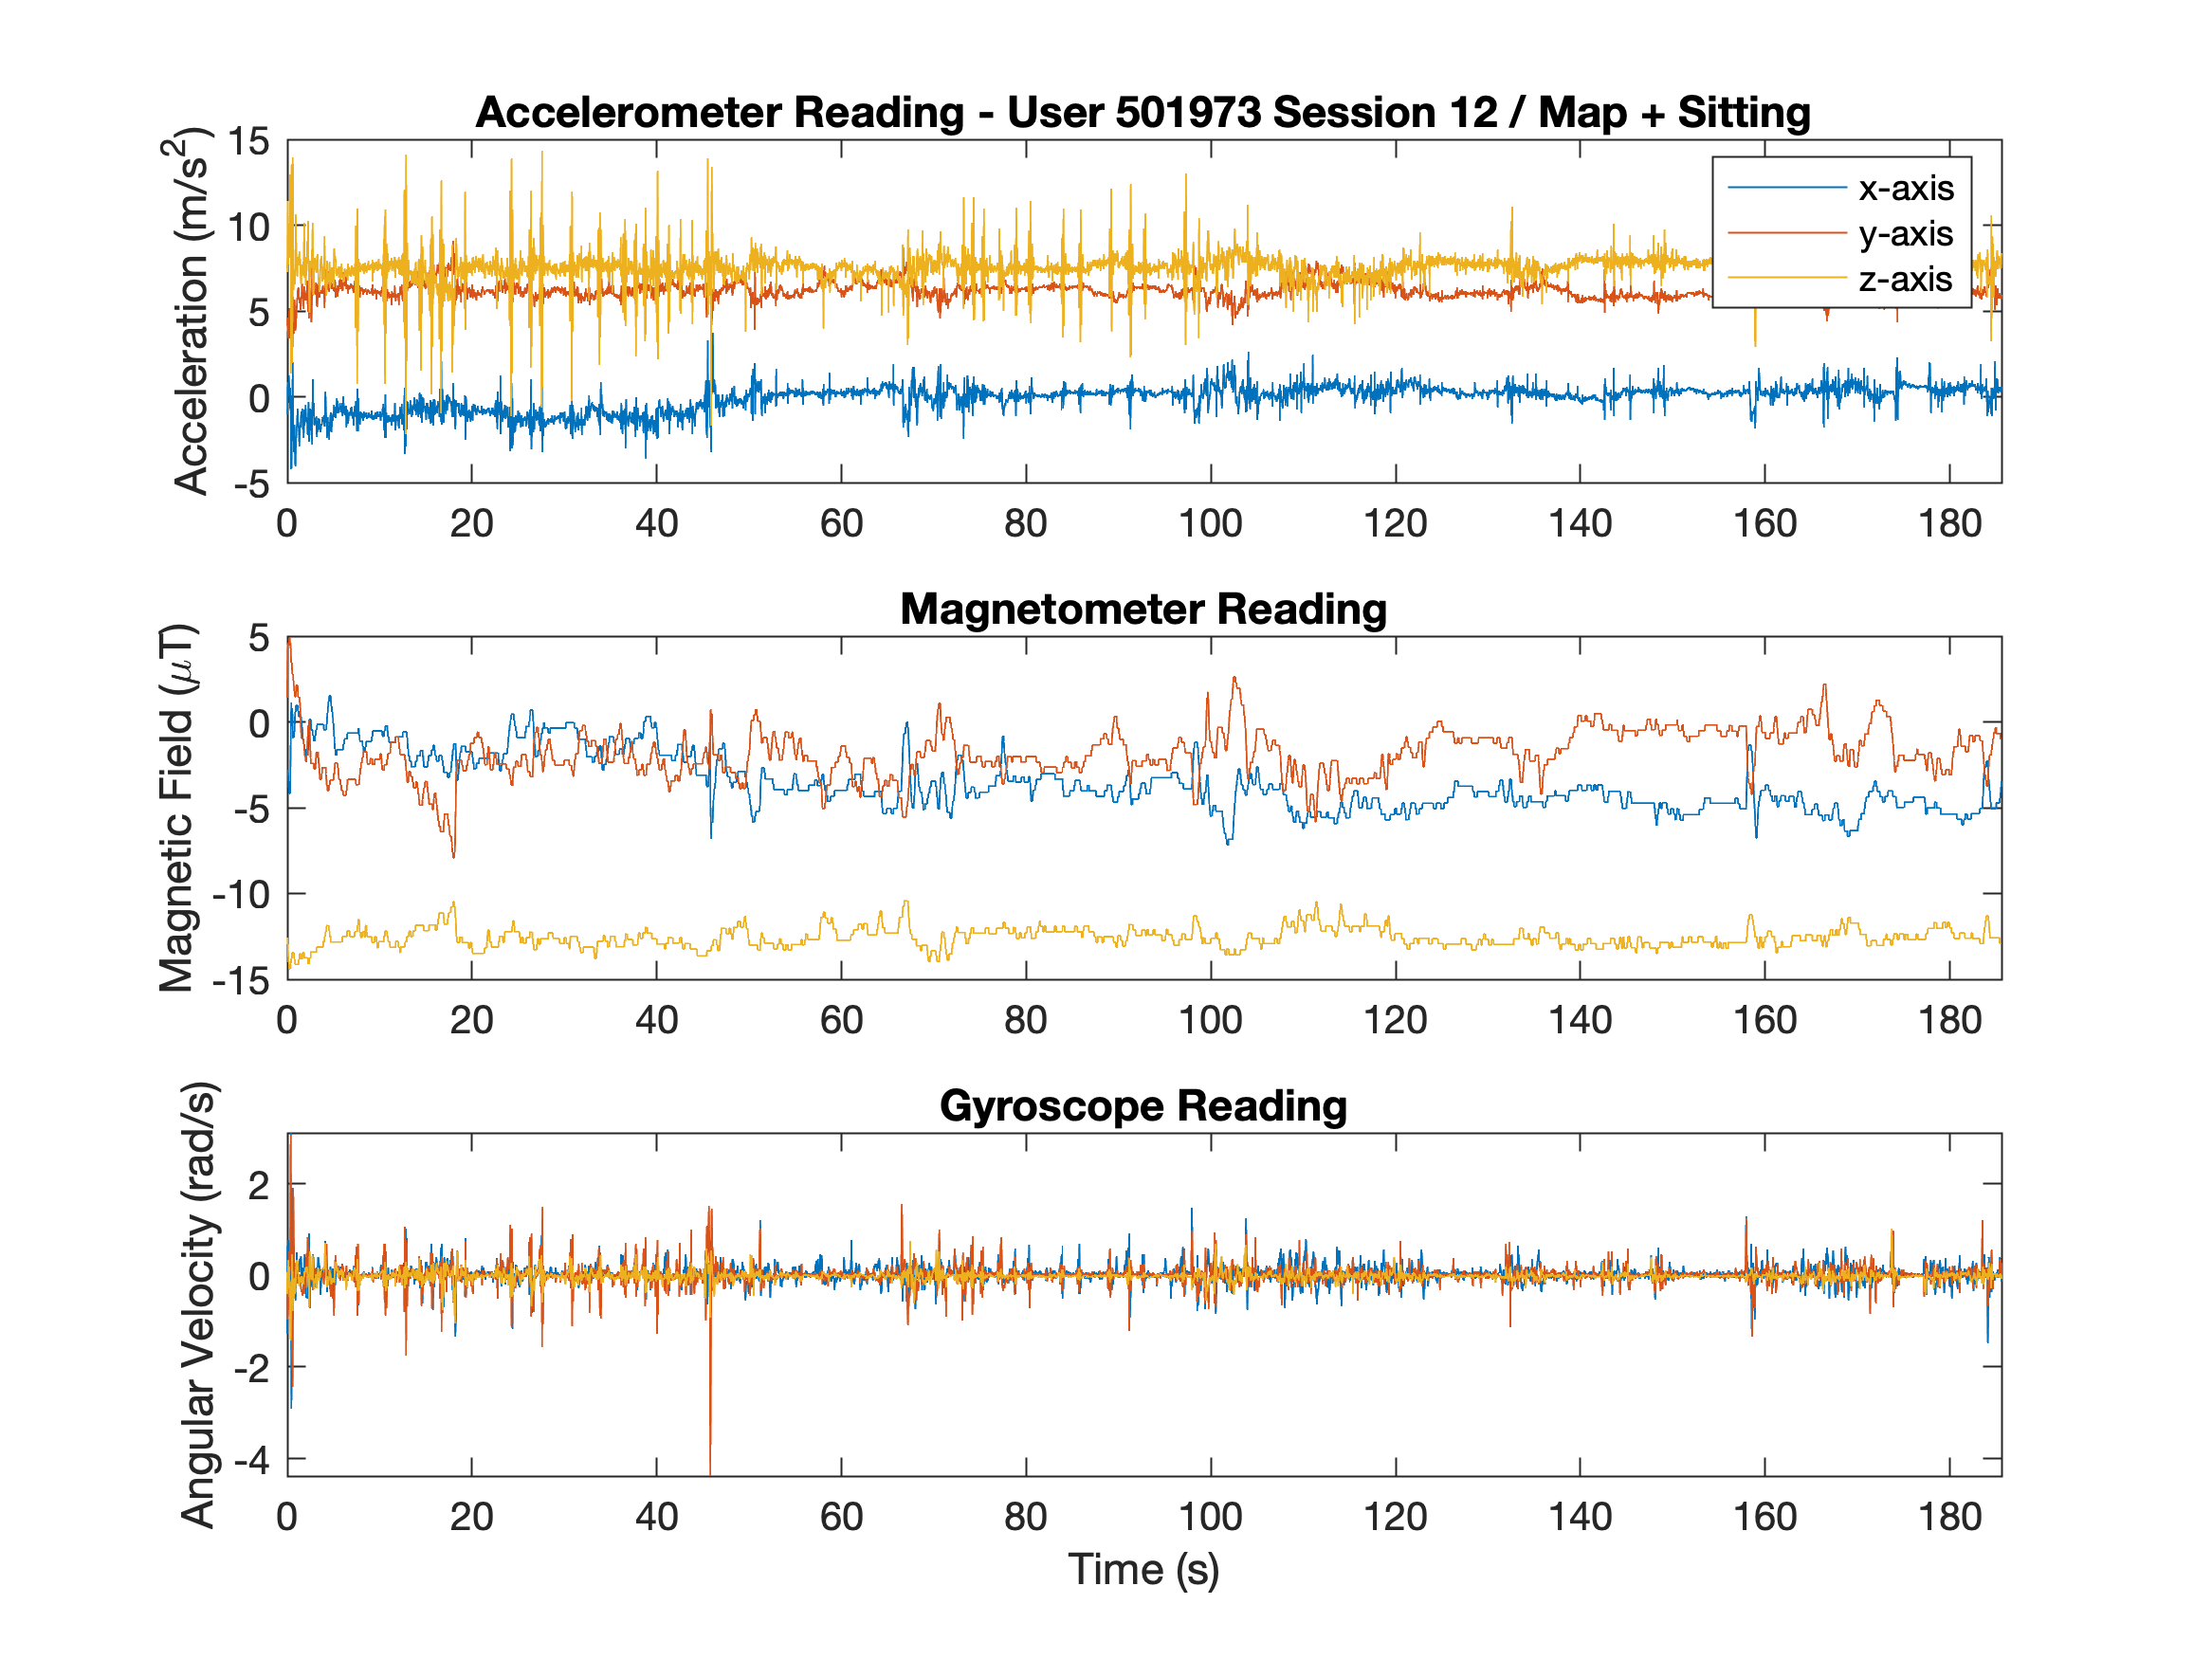
\includegraphics[width=1\linewidth]{images/501973_12_acc_mag_gyr_data.png}
  \caption[]{HMOG cell phone IMU data.}
  %
  \label{fig:501973_12_imu}
\end{figure}

\begin{figure}[ht]
  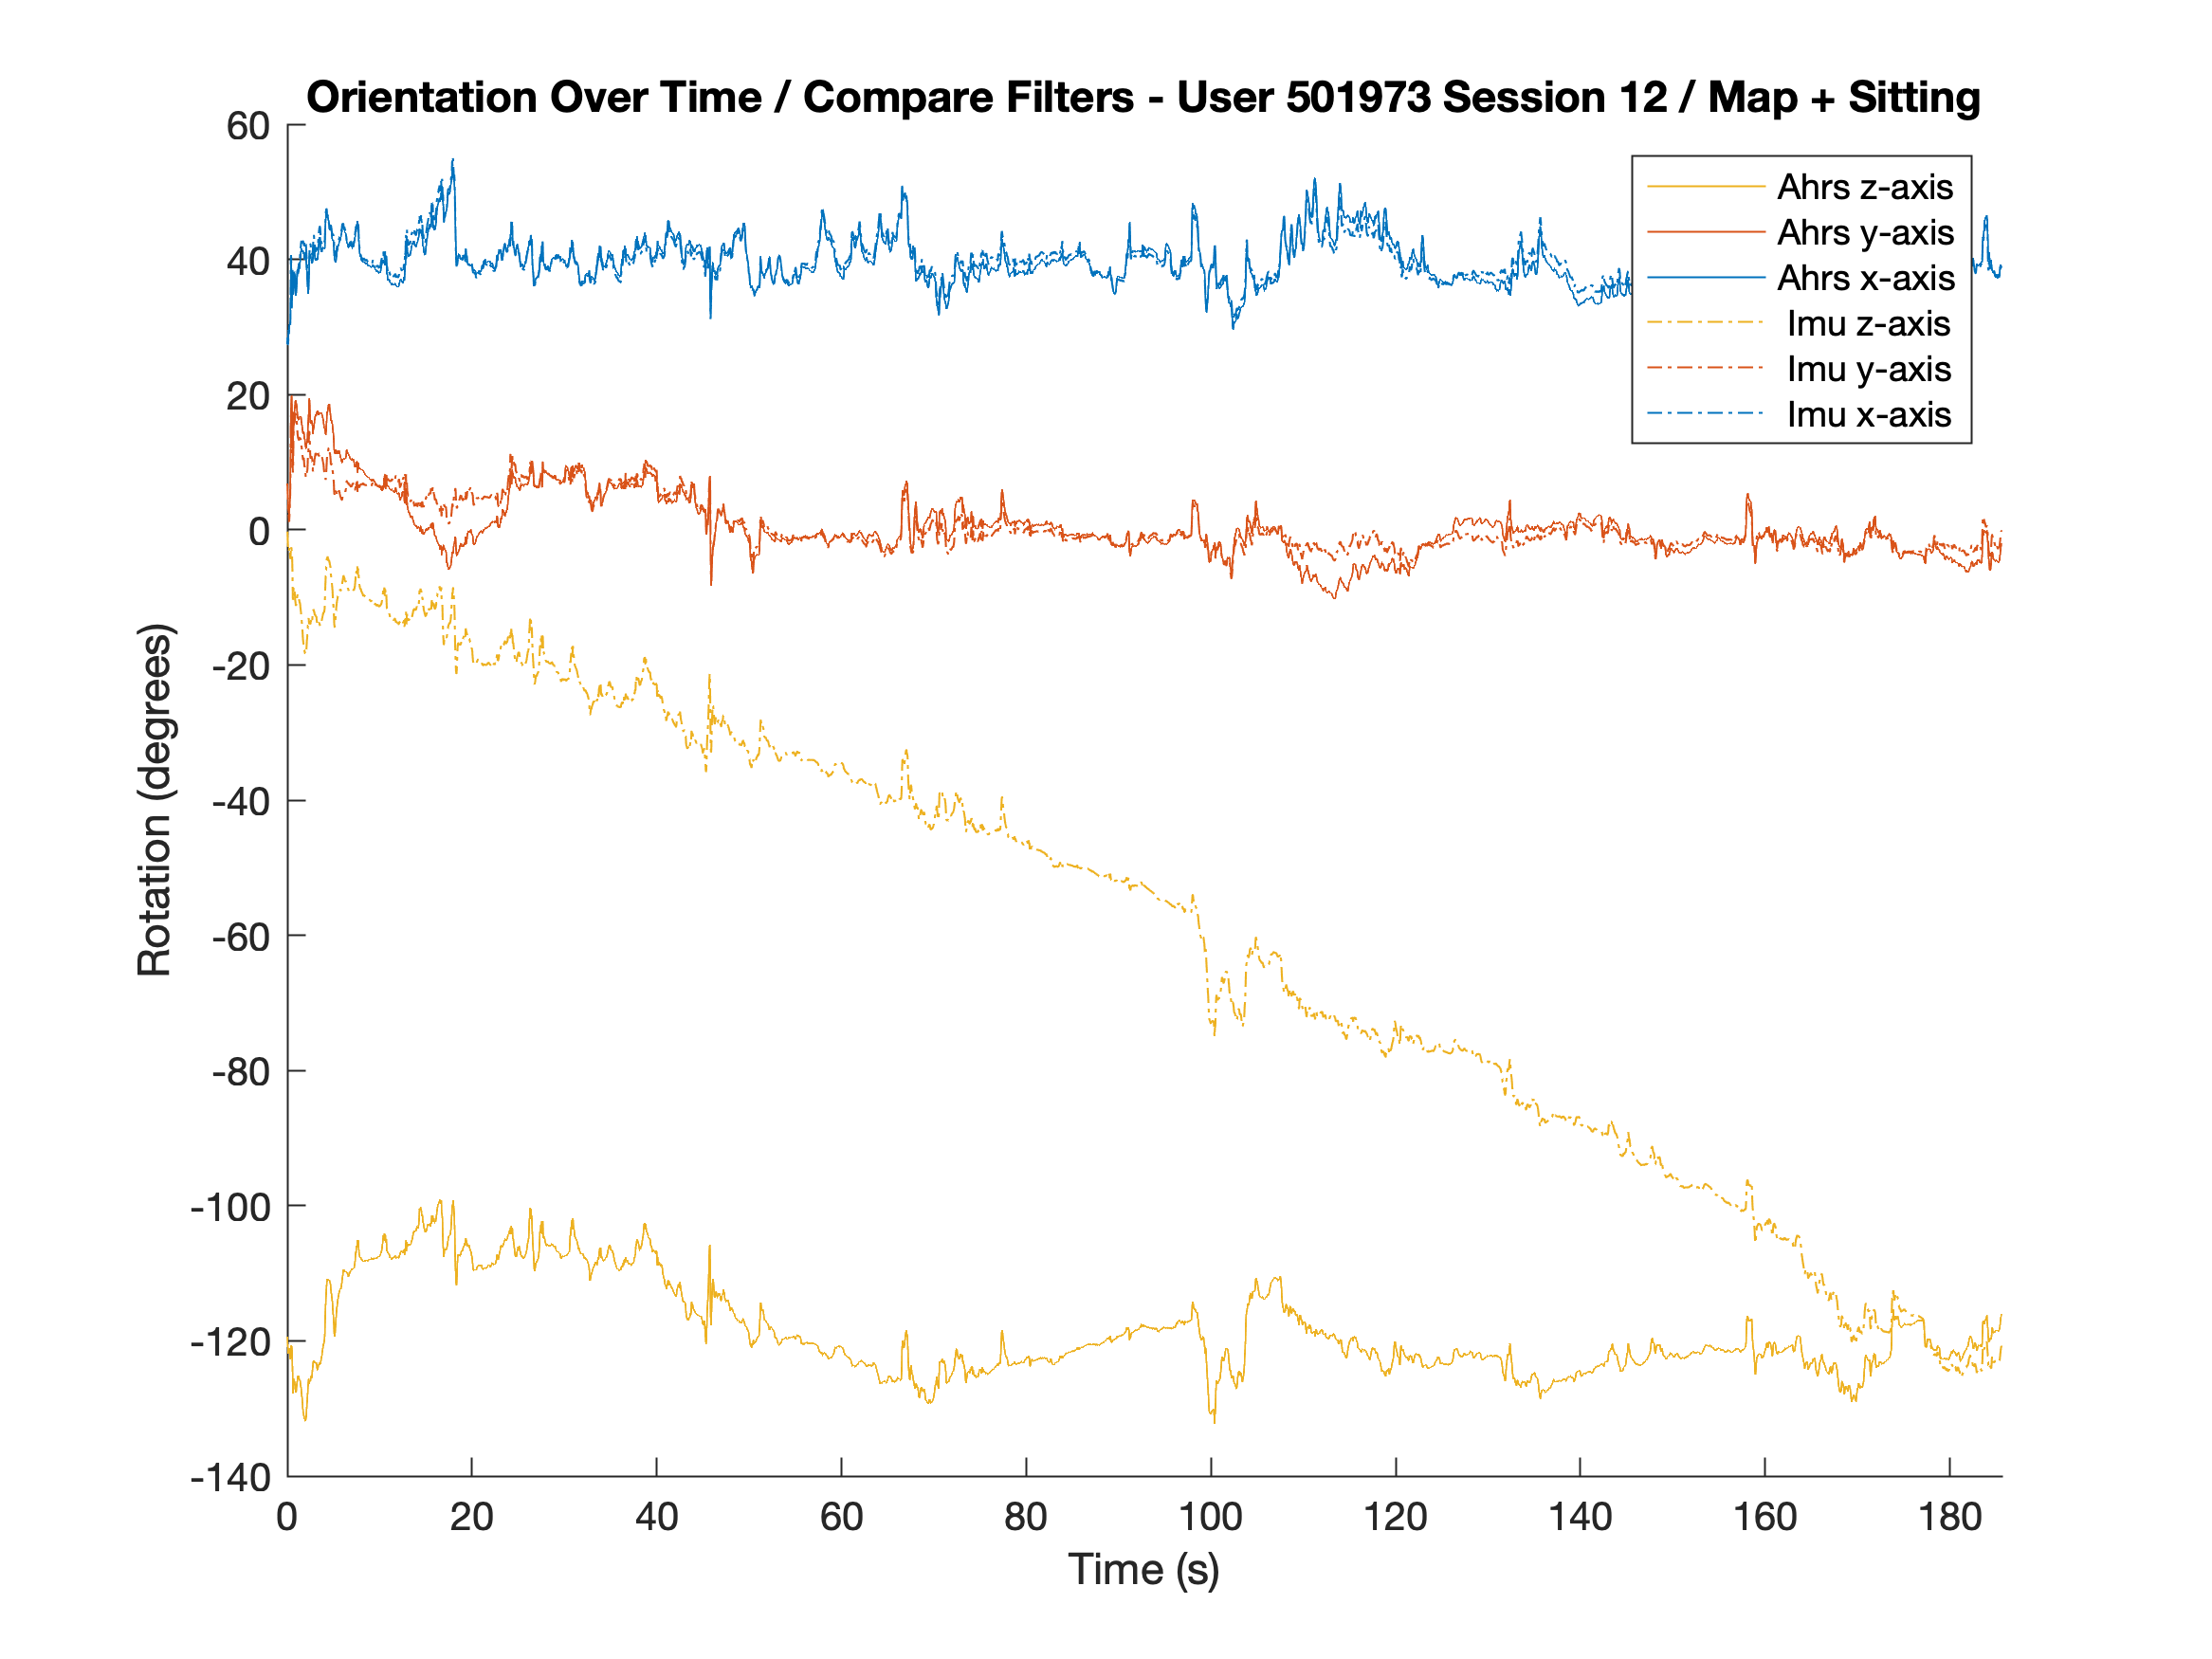
\includegraphics[width=1\linewidth]{images/501973_12_orientation_compare_filters.png}
  \caption[]{Comparison Matlab AHRS and IMU filtering algorithms.}
  %
  \label{fig:501973_12_compare_filter}
\end{figure}

\begin{figure}[ht]
  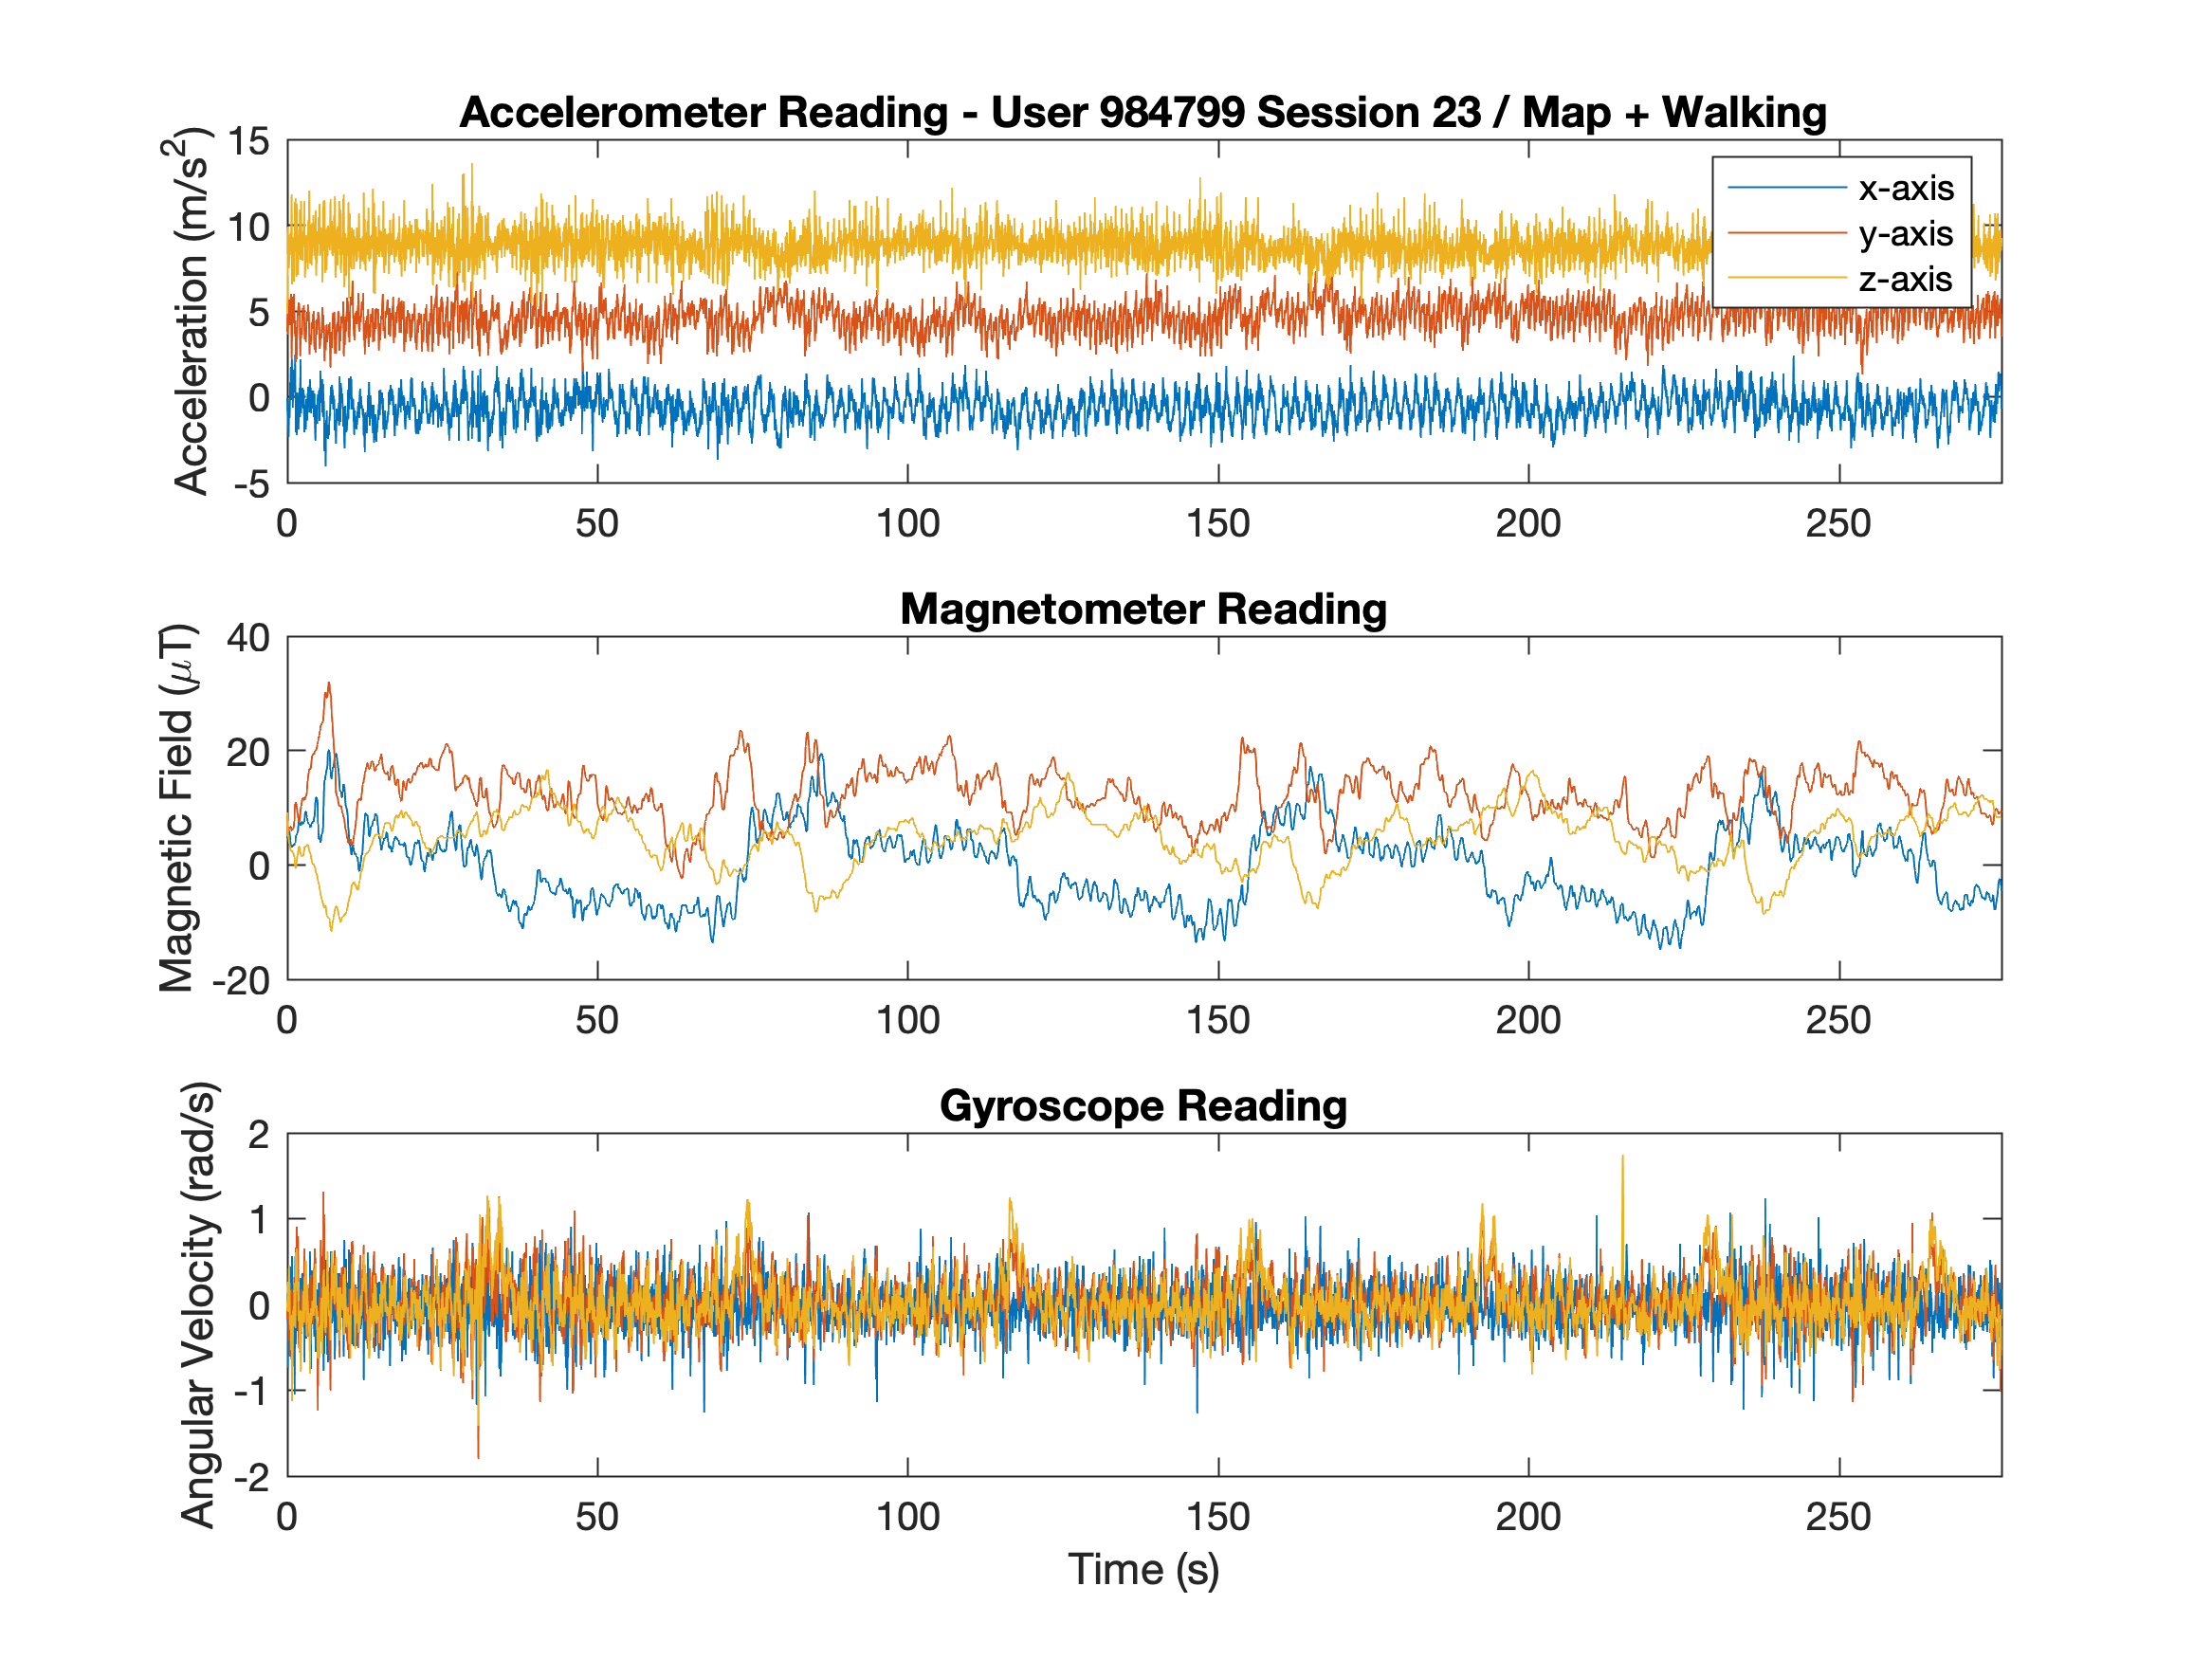
\includegraphics[width=1\linewidth]{images/984799_23_acc_mag_gyr_data.png}
  \caption[]{HMOG cell phone IMU data.}
  %
  \label{fig:984799_23_imu}
\end{figure}

\begin{figure}[ht]
  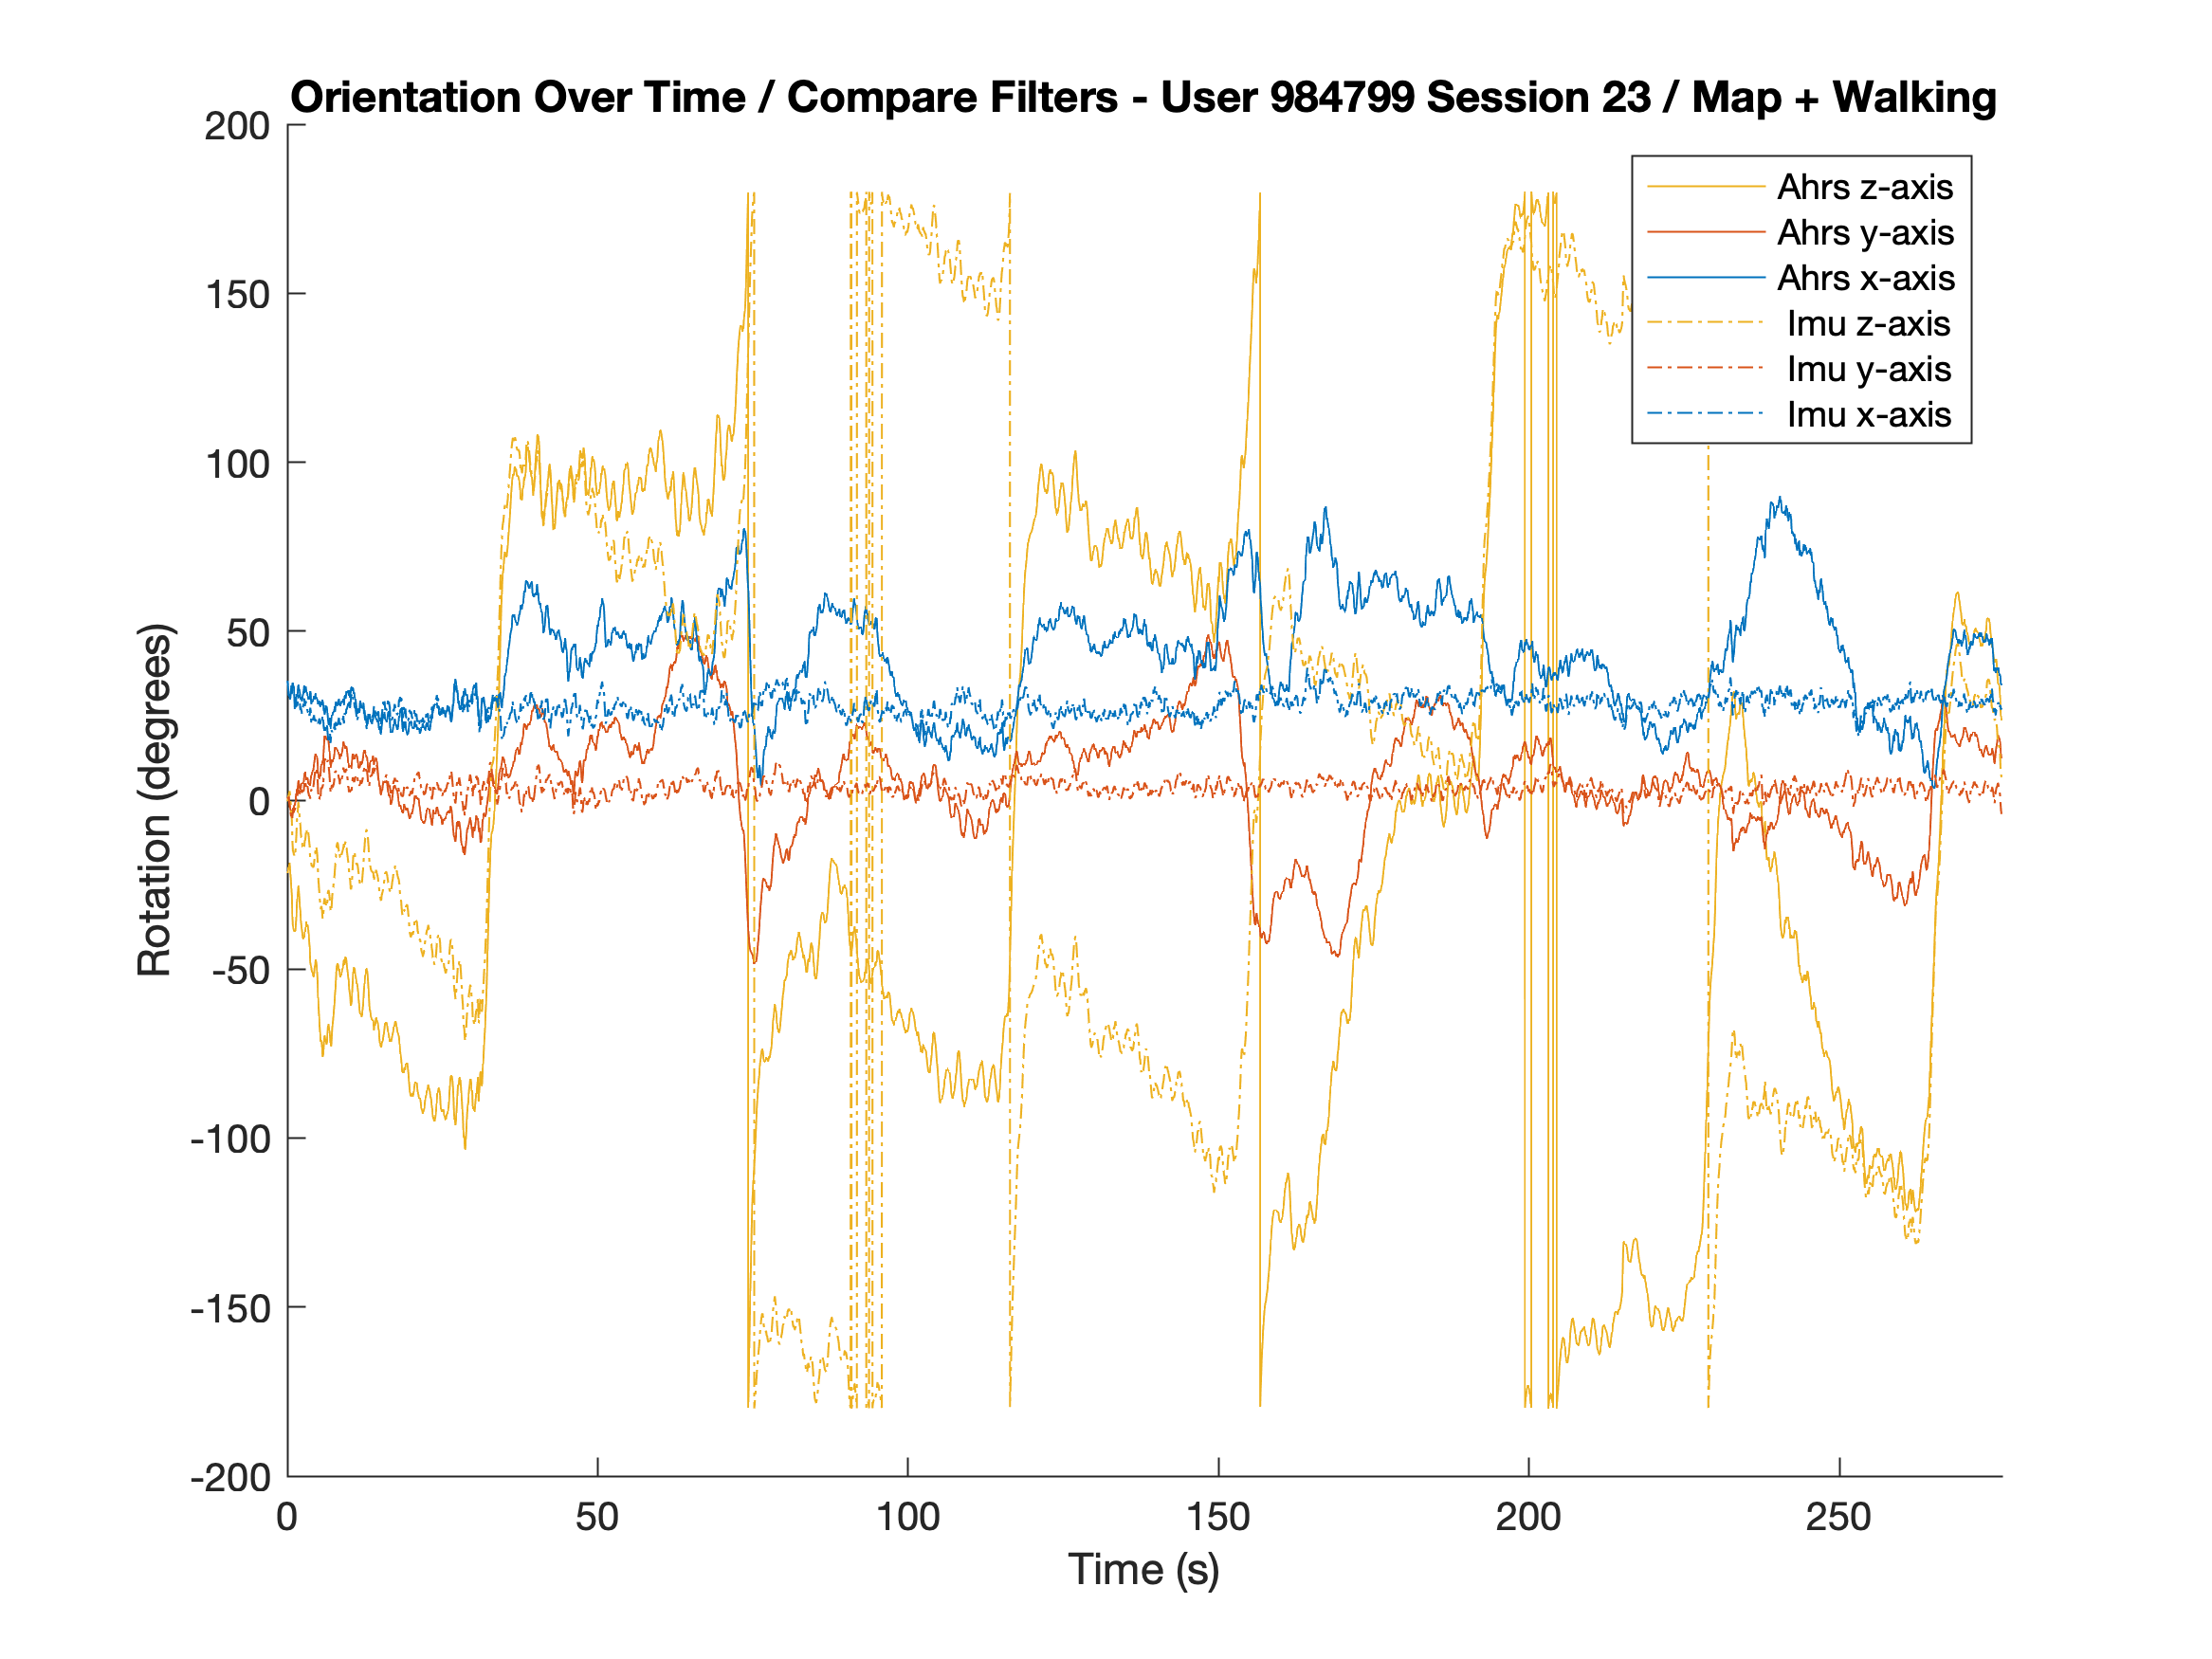
\includegraphics[width=1\linewidth]{images/984799_23_orientation_compare_filters.png}
  \caption[]{Comparison Matlab AHRS and IMU filtering algorithms.}
  %
  \label{fig:984799_23_compare_filter}
\end{figure}

\subsection{Python Scikit Kinematics Library}












\subsection{Conclusion and further work}






















\section*{References}

\small

[1] Manon Kok, Jeroen D. Hol and Thomas B. Schon (2017), Using
Inertial Sensors for Position and Orientation Estimation,
{\it Foundations and Trends in Signal Processing: Vol. 11: No. 1-2},
pp 1-153. \\ \url{http://dx.doi.org/10.1561/2000000094}

[2] SITOVÁ, Zdeňka, Jaroslav ŠEDĚNKA, Qing YANG, Ge PENG, Gang ZHOU,
Paolo GASTI and Kiran BALAGANI. HMOG: New Behavioral Biometric Features
for Continuous Authentication of Smartphone Users. {\it IEEE Transactions on
Information Forensics and Security, 2016, Vol. 11, No. 5}, p. 877 - 892.
ISSN 1556-6013. \\ \url{http://dx.doi.org/10.1109/TIFS.2015.2506542}

[3] MATLAB Sensor Fustion and Tracking Toolbox. \\ \url{https://www.mathworks.com/help/fusion/}

[4] Scikit Kinematics Library. \\ \url{http://work.thaslwanter.at/skinematics/html}

[5] Open Source Sensor Fusion. \\ \url{https://github.com/memsindustrygroup/Open-Source-Sensor-Fusion/tree/master/docs}

\end{document}
